% !TEX root = ./Basilisk-CoarseSunSensor-20170803.tex

\section{Test Description and Success Criteria}
The Coarse Sun Sensor Test, test\_coarseSunSensor.py, contains 11 tests. The simulation is set up with only the coarse sun sensor(s) and made-up messages to simulation spacecraft, sun, and eclipse information. The spacecraft is in a convenient attitude relative to the sun and rotates all of the sensors in a full circle past the sun.
\begin{enumerate}
	\item\textbf{Basic Functionality}: A single sensor is run with minimal modifications and compared to a cosine.
	\subitem \textbf{Success Criteria}: The output curve should match a cosine curve.
	\item\textbf{Eclipse}: A single sensor is run with an eclipse simulated and compared to an eclipse factored cosine.
	\subitem \textbf{Success Criteria}: The output curve should match a cosine curve times the eclipse factor input
	\item\textbf{Field of View}: A single sensor is run with a smaller field of view and compared to a clipped cosine.
	\subitem \textbf{Success Criteria}: The output curve should match a cosine curve truncated to zero beyond the field of view input.
	\item\textbf{Kelly Factor}: A single sensor is run with a Kelly factor input and compared to a modified cosine.
	\subitem \textbf{Success Criteria}: The output curve should match a cosine curve modified by the kelly curve equation seen previously in this report
	\item\textbf{Scale Factor}: A single sensor is run with a scale factor and compared to a scaled cosine.
	\subitem \textbf{Success Criteria}: The output curve should match a cosine curve multiplied by the scaleFactor input.
	\item\textbf{Bias}: A single sensor is run with a bias and compared to a modified cosine.
	\subitem \textbf{Success Criteria}: The output curve should match a cosine curve shifted in magnitude by the bias input.
	\item\textbf{Noise}: A single sensor is run with noise and the standard deviation of that noise is compared to the input standard deviation.
	\subitem \textbf{Success Criteria}: Once a clean cosine curve is subtracted from the output, the standard deviation should match the standard deviation input.
	\item\textbf{Albedo}: A single sensor is run with an albedo input and shown to be no different than the standard cosine truth value. This is done because there is some albedo functionality programmed into the module but it should be inactive at this time.
	\subitem \textbf{Success Criteria}: The output curve should match a cosine curve because the albedo input should have no effect.
	\item \textbf{Saturation}: Non-zero minimum saturation and less-than-maximum-output maximum saturation values are input.
	\subitem\textbf{SuccessCriteria}: Output should match generated truth to high accuracy and saturation values should be clearly visible in plot.
	\item\textbf{Sun Distance}: The simulation is run with the spacecraft $2[AU]$ from the sun. The expected result is compared to the output.
	\subitem \textbf{Success Criteria}: Output should match the generated truth to high accuracy.
	\item\textbf{Clean Combined}: All of the inputs above except for noise are run on a single simulation. The expected result is compared to the output.
	\subitem \textbf{Success Criteria}: Output should match the generated truth to high accuracy.
	\item\textbf{Combined}: All of the inputs above are run on a single simulation. The expected result without noise is subtracted from the result. Then, the standard deviation of the noise. is compared to the expected standard deviation.
	\subitem \textbf{Success Criteria}: Once a cosine curve modified by eclipse, field of view, kelly factor, scale factor, bias, and albedo are subtracted from the output, the standard deviation should match the given standard deviation.
	\item\textbf{Constellation}: Two constellations of sensors are set up using various set up methods and simulated with a clean signal. The two constellations are tested to be identical to one another. Constellation P1 is established by directly assigning normal vectors to four sensors. Constellation P2 is established by giving angles that specify the placement of the constellation platform relative to the spacecraft body frame. Then, for constellation 2, the unit direction vector for each sensor is set with an azimuth and an elevation via coarseSunSensor.setUnitDirectionVectorWithPerturbation(). Finally, the fourth sensor in constellation P2 is set up in a different way than the others. It is not assigned platform frame angles but it is given incorrect azimuth and elevation headings which are corrected with "perturbation" inputs. Through all of these tests, constellation set up is verified, including the default platform DCM (identity).
	\subitem \textbf{Success Criteria}: The output curve from constellation P1 should match the output curve from constellation P2.
\end{enumerate}


\section{Test Parameters}

Pytest runs the following cases (numbered as above) when it is called for this test:
	\begin{table}[H]
	\caption{Parameters for each test. Note that relative tolerance is $\frac{truth - output}{truth}$}
	\label{tab:errortol}
	\centering \fontsize{10}{10}\selectfont
	\begin{tabular}{ c | c | c | c | c | c | c | c | c | c | c | c } % Column formatting, 
		\hline\hline
		\rot{\textbf{Test}}& \rot{\textbf{useConstellation}}& \rot{\textbf{visibilityFactor}}& \rot{\textbf{fov}}& \rot{\textbf{kelly}}& \rot{\textbf{scaleFactor}}& \rot{\textbf{bias}}& \rot{\textbf{noiseStd}}& \rot{\textbf{albedoValue}}& \rot{\textbf{saturation}}&\rot{\textbf{errTol}}&\rot{\textbf{sunDistInput}}\\ 
		\hline\hline
		1      & False&1.00&1.5708&0.00&1.00&0.00&0.000&0.0&10.00,0.00&1.0e-10&1.0	   \\ \hline
		2	& False&0.50&1.5708&0.00&1.00&0.00&0.000&0.0&10.00,0.00&1.0e-10&1.0	   \\ \hline
		3	& False&1.00&1.1781&0.00&1.00&0.00&0.000&0.0&10.00,0.00&1.0e-10&1.0	   \\ \hline
		4      & False&1.00&1.5708&0.15&1.00&0.00&0.000&0.0&10.00,0.00&1.0e-10&1.0	   \\ \hline
		5	& False&1.00&1.5708&0.00&2.00&0.00&0.000&0.0&10.00,0.00&1.0e-10&1.0	   \\ \hline
		6 & False&1.00&1.5708&0.00&1.00&0.50&0.000&0.0&10.00,0.00&1.0e-10&1.0	   \\ \hline
		7    & False&1.00&1.5708&0.00&1.00&0.00&0.125&0.0&10.00,-10.00&3.0e-02&1.0	   \\ \hline
		8	& False&1.00&1.5708&0.00&1.00&0.00&0.000&0.5&10.00,0.00&1.0e-10&1.0	   \\ \hline
		9	& False&1.00&1.5708&0.00&1.00&0.00&0.000&0.0&0.75,0.25&1.0e-10&1.0	   \\ \hline
		10	& False&1.00&1.5708&0.00&1.00&0.00&0.000&0.0&10.00,0.00&1.0e-10&2.0	   \\ \hline
		11	& False&0.50&1.1781&0.15&2.00&0.50&0.000&0.5&10.00,0.00&1.0e-10&2.0	   \\ \hline
		12	& False&0.50&1.1781&0.15&2.00&0.50&0.125&0.5&10.00,-10.00&3.0e-02&2.0	   \\ \hline
		13    & True&1.00&1.5708&0.00&1.00&0.00&0.000&0.0&10.00,0.00&1.0e-10&1.0	   \\ \hline
		\hline
	\end{tabular}
\end{table}
The tolerances above were chosen basically to be machine tolerance which is consistently passable between machines and operating systems. Those tests involving noise have looser tolerances because they are comparing the standard deviation of generated noise with the requested standard deviation. longer runs would make this tolerance tighter, but take large amounts of time for users to run the tests.

\section{Test Results}
The results of each test are shown in the table below. If a test did not pass, an error message is included.

\begin{table}[H]
	\caption{Test results.}
	\label{tab:results}
	\centering \fontsize{10}{10}\selectfont
	\begin{tabular}{ c | c | c } % Column formatting, 
		\hline
		\textbf{Test} & \textbf{Pass/Fail} 						   		    			& \textbf{Notes} 									      \\ \hline
		1	   			  	&\textcolor{ForestGreen}{PASSED}      	   			&\input{AutoTex/plainPassFailMsg} 	         	\\ \hline
		2	   			  	&\textcolor{ForestGreen}{PASSED}       			&\input{AutoTex/eclipsePassFailMsg} 	       \\ \hline
		3	   			  	&\textcolor{ForestGreen}{PASSED}			&\input{AutoTex/fieldOfViewPassFailMsg} 	 \\ \hline
		4	   			  	&\textcolor{ForestGreen}{PASSED} 			&\input{AutoTex/kellyFactorPassFailMsg} 	   \\ \hline
		5	   			  	&\textcolor{ForestGreen}{PASSED}			&\input{AutoTex/scaleFactorPassFailMsg} 	 \\ \hline
		6	   			  	&\textcolor{ForestGreen}{PASSED}      	  			&\input{AutoTex/biasPassFailMsg} 	              \\ \hline
		7	   			  	&\textcolor{ForestGreen}{PASSED}    		&\input{AutoTex/deviationPassFailMsg} 	     	 \\ \hline
		8	   			  	&\textcolor{ForestGreen}{PASSED}      			&\input{AutoTex/albedoPassFailMsg} 	           		\\ \hline
		9	   			  	&\textcolor{ForestGreen}{PASSED} 			&\input{AutoTex/saturationPassFailMsg} 	        \\ \hline
		10	   			  	&\textcolor{ForestGreen}{PASSED}      &\input{AutoTex/sunDistancePassFailMsg} 	   \\ \hline
		11	   			  	&\textcolor{ForestGreen}{PASSED}    &\input{AutoTex/cleanCombinedPassFailMsg} \\ \hline
		12	   			  	&\textcolor{ForestGreen}{PASSED}  		&\input{AutoTex/combinedPassFailMsg} 	      	\\ \hline
		13	   			  	&\textcolor{ForestGreen}{PASSED} 	&\input{AutoTex/constellationPassFailMsg}		\\ \hline
	
	\end{tabular}
\end{table}

In addition to the tabulated results, test data has been plotted for visual inspection. In Fig. \ref{fig:combinedPlot}, all single coarse sun sensor simulations have been plotted on top of one another. This makes for convenient comparison between the cases. For instance, the scaleFactor case can be seen to peak at 2 rather than 1 whereas the eclipse case peaks at 0.5. Furthermore, the fieldOfView test drops to zero at a value less than $\frac{\pi}{2}$ but it follows the plain case otherwise. The kellyFactor case similarly follows the plain curve, except at the edges. The albedo curve cannot be seen because it lies directly beneath the plain curve. The bias curve is equivalent to the plain curve, but shifted up. Finally, the two curves with noise clearly follow the ordinary curve pattern.

\begin{figure}[htbp]\centerline{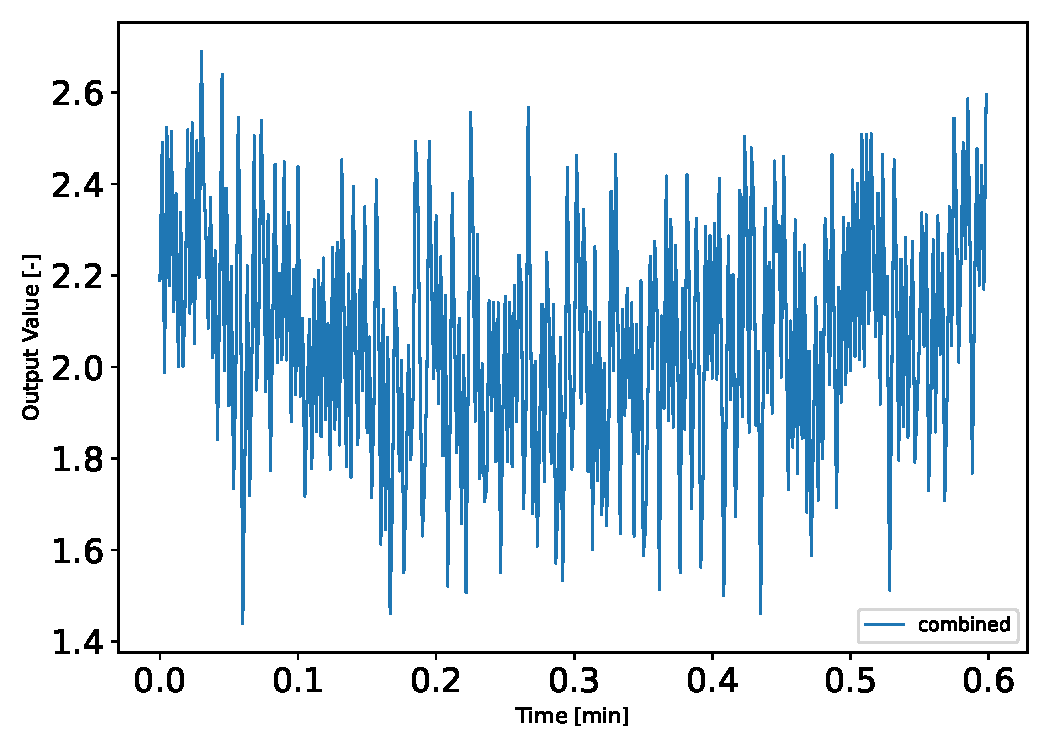
\includegraphics[height=0.7\textwidth, keepaspectratio]{AutoTeX/combinedPlot}}\caption{Plot of all cases of individual coarse sun sensor in comparison to                                              each other. Note that the incidence angle starts at direct and linearly                                               rotates in time until it returns to a direct view.}\label{fig:combinedPlot}\end{figure}
\clearpage
The constellation test results are shown in Fig. \ref{fig:constellationPlots}. The results are identical to each other and the test has been successful.

\begin{figure}[htbp]\centerline{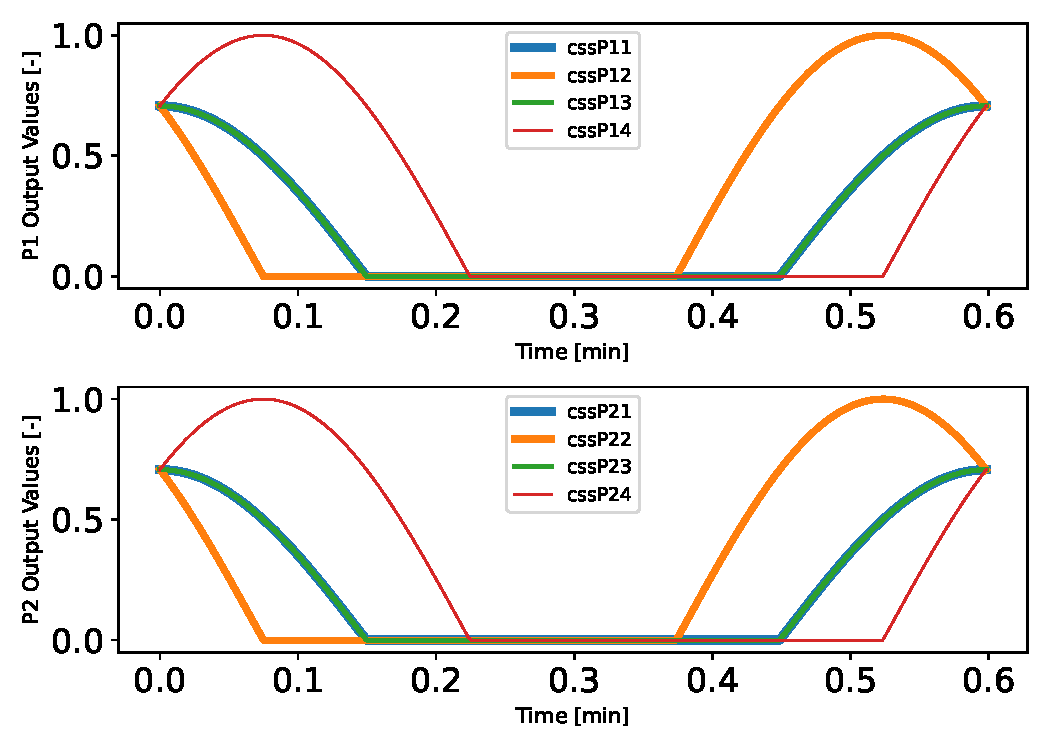
\includegraphics[height=0.7\textwidth, keepaspectratio]{AutoTeX/constellationPlots}}\caption{Plot of first and second constellation outputs for comparision.                                          Note that the constellation starts pointing directly at the sun                                           and linearly rotates in time until it returns to a direct view.}\label{fig:constellationPlots}\end{figure}
